\documentclass[UTF8]{ctexart}

\usepackage{amsmath}
\usepackage{float}
\usepackage{cases}
\usepackage{cite}
\usepackage{graphicx}
\usepackage[margin=1in]{geometry}
\geometry{a4paper}
\usepackage{fancyhdr}
\usepackage{booktabs}
\pagestyle{fancy}
\fancyhf{}


\title{$KNO_3$溶解热的测定}
\author{522111910161 尚子翔}
\date{\today}
\pagenumbering{arabic}

\begin{document}

\fancyhead[L]{}
\fancyhead[C]{$KNO_3$溶解热的测定}
\fancyfoot[R]{\thepage}

\maketitle
\tableofcontents
\newpage

\section{实验目的}
\begin{enumerate}
    \item 了解热效应测定的基本原理。 
    \item 掌握摩尔积分溶解热、摩尔微分溶解热、摩尔积分稀释热和摩尔微分稀释热的定义。
    \item 使用电热补偿法借助微机控制测定硝酸钾在水中的积分溶解热。
    \item 使用作图法求出硝酸钾在水中的微分溶解热,积分冲淡热和微分冲淡热。
\end{enumerate}



\section{实验原理}
恒温恒压下1mol纯物质溶解于一定量的溶剂中形成溶液时所产生的热效应称为此物质在该条件下的摩尔积分溶解热,用$\Delta_{sol}H_m$表示。摩尔积分溶解热不仅与溶质溶剂的本性有关,而且还与所形成溶液的浓度有关。随着溶液浓度减小,摩尔积分溶解热趋于定值,此值称为该物质的无限稀释摩尔积分溶解热。物质在25℃时以水为溶剂的无限稀释摩尔积分溶解热可从手册中查得。恒温恒压下,在一定量某浓度的溶液中加入$dn_2$量的溶质,产生的热效应$d(\Delta_{sol}H_m)$与$dn_2$之比称为摩尔微分溶解热。由于加入溶质的量为$dn_2$,可以认为溶液的浓度不变。因此,摩尔微分溶解热亦可以认为是在一定浓度的大量溶液中加入1mol溶质所产生的热效应。

恒温恒压下,将一定量溶剂加入到含1mol溶质的溶液中形成较稀溶液时的热效应为摩尔积分稀释热或摩尔积分冲淡热,用$\Delta d_{il}H_m$表示。摩尔积分稀释热为稀释前后溶液的摩尔积分溶解热之差$\Delta d_{il}H_m=\Delta_{sol}H_m(2)-\Delta_{sol}H_m(1)$若加入溶剂的量为$dn_1$,则产生的热效应$d(\Delta_{sol}H_m)$与$dn_1$之比称为摩尔微分稀释热或摩尔微分冲淡热。显然摩尔积分稀释热和摩尔微分稀释热均与所形成溶液的浓度有关。

无机盐类的溶解通常包含晶格的破坏和离子的溶剂化两个过程。前者为吸热过程,后者为放热过程,盐类的溶解热是这两种热效应的总和。测量盐类的溶解热是在绝热式热量计中进行的。本实验测定硝酸钾在水中的溶解热,由于硝酸钾的溶解过程为吸热过程,故根据电热补偿法原理采用NDRH-2S型微机测定溶解热实验系统进行溶解过程热量测定,该系统能自动完成$KNO_3$溶解热实验数据的测量、记录及处理全过程。该系统主要由系统软件和热量测定两部分构成,基本装置如下图所示。

其原理为先测定含有确定量水的绝热体系的起始温度T,在绝热恒压条件下向水中加人一定质量的硝酸钾,随着溶解过程的不断进行,体系的温度不断下降,为了使体系回复到实验前的起始温度需要不断由电热丝加热体系,根据所消耗的电能便可求出溶解过程的热效应$Q=PRE=IVt$式中:1为通过电阻为R的电热丝的电流强度,V为电热丝两端所加的电压,t为通电时间,此Q值即为所加人硝酸钾在此溶解过程中吸收的热量。

根据摩尔据摩尔积分溶解热的定义,硝酸钾的摩尔积分溶解热$\Delta_{sol}H_m=\frac{Q}{KNO_3}$。若定义溶解每摩尔硝酸钾所用水的量$n_0=\frac{n_{H_2O}}{n_{KNO_3}}$则由实验测定不同$n_0$下的$\Delta_{sol}H_m$可作下图。

\begin{figure}[H]
  \centering
  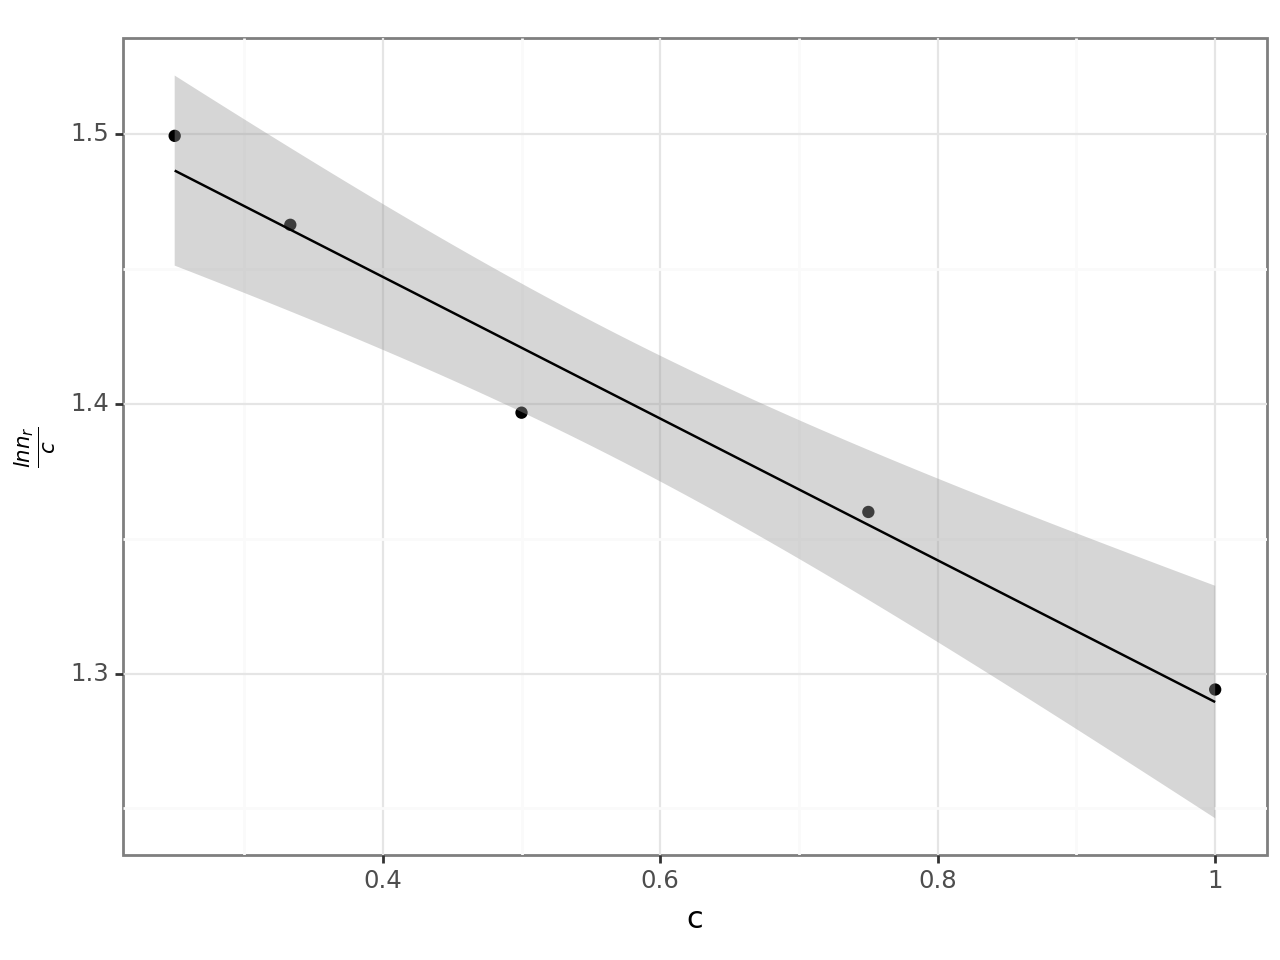
\includegraphics[scale = 0.1]{fig1.JPG} % 图片文件的名称和路径
  \caption{硝酸钾在水中的摩尔积分溶解热曲线}
  \label{fig:example}
\end{figure}

若将纯溶剂和纯溶质的摩尔焓分别表示为$H_m(1)$和$H_m(2)$,溶液中溶剂和溶质的偏摩尔焓分别表示为$H_{1,m}$和$H_{2,m}$,则恒压下将$n_2$量的溶质溶解于$n_1$量的溶剂时,过程的热效应

\[Q=\Delta H=n_1H_{1,m}+n_2H_{2,m}-[n_1H_m(1)+n_2H_m(2)]=n_1\Delta H_m(1)+n_2\Delta H_m(2)\]

式中Δ$H_m$(1)为摩尔微分稀释热,Δ$H_m$(2)为摩尔微分溶解热。

由摩尔积分溶解热的定义得
\[\Delta_{sol}H_m=\frac{\Delta H}{n_2}=\frac{n_1}{n_2}\Delta H_m(1)+\Delta H_m(2)=n_0\Delta H_m(1)+\Delta H_m(2)\]

在摩尔积分溶解热曲线图中,不同$n_0$点对应的切线斜率为该浓度下溶液的摩尔微分稀释热。即在上图中,A点对应浓度下的摩尔微分稀释热\[\left[ \frac{ \partial\Delta_{sol}H_m}{\partial n_0}\right] _{T,p,n_2} = \frac{AC}{BC}\]该切线在纵坐标上的截距OB即为对应于该浓度溶液的摩尔微分溶解热。

在含有1mol溶质的溶液中加入溶剂所产生的摩尔积分稀释热,就是两浓度下积分溶解热的差值。即在图2.1.2中,由A点相应浓度稀释至E点相应浓度,过程的摩尔积分稀释热$\Delta d_{il}H_m=EG-AF$

\section{实验步骤}
\subsection{仪器与试剂}
\begin{itemize}
    \item NDRH-2S型微机测定溶解热实验系统1套
    \item 计算机1台
    \item 最大称量为101g和610g的电子天平各1台
    \item 20x40mm称量瓶8个
    \item 毛笔1支
    \item 洗瓶1只
    \item 经研细与110℃烘干的硝酸钾(A.R.)
\end{itemize}

\subsection{操作流程}
\begin{enumerate}
    \item 依次在最大称量为101g的电子天平上准确称取2.5,1.5,2.5,3.0,3.5,4.0和4.5g$KNO_3$样品于已标号的称量瓶中。注意称量过程应盖上称量瓶盖子以防止样品吸潮,盛有样品的称量瓶应放人干燥器中备用。在最大称量为610g的电子天平上准确称取216.2g去离子水于干净干燥的保温杯中备用。
    \item 打开 NDRH-2S型微机测定溶解热实验系统电源,预热10min。
    \item 启动计算机至桌面状态。点击“溶解热数据测量系统”,进入系统界面,再点击“继续”,出现反应热测量系统界面,在上方的菜单栏点击“开始实验”,之后继续点击“开始实验”按钮,将干净、干燥的温度传感器置于空气中,此时系统开始自动测量室温。
    \item 待室温稳定后将温差置零,开启磁力搅拌器电源,调节磁力搅拌至中等速率,搅拌去离子水。根据计算机提示将加热装置连同温度传感器等一起置于保温杯内中的去离子水中,注意温度传感器探头不要与搅拌磁子和加热电热丝相接触。调节恒流电源,使加热器功率在2.25W到2.3W之间。此时体系开始升温。
    \item 当温度传感器采样到水温高于室温0.5℃时,计算机提示加入第一份$KNO_3$样品,加入后记录下加热器功率,同时计算机会实时记下此时水温和加热开始时间。加入$KNO_3$样品后,由于样品溶解吸热使水温下降,电热丝的加热使水温回升。当温度传感器探测到水温回升至第一份样品加入前的温度时,计算机提示加入第二份$KNO_3$样品,同时计算机给出第一份$KNO_3$样品溶解过程中的电热补偿通电时间。按计算机提示重复加样操作,直至加完8份$KNO_3$样品,计算机显示实验完成为止。注意,样品加入应少量连续,防止加样管被样品堵塞,每次加样后用毛笔将称量瓶和加样漏斗上残留的样品刷入加样孔。
    \item 加样结束后按计算机提示点击对话框右下方的“退出”按钮退出实验。将NDRH-2S型微机测定溶解热实验系统的电流调节旋钮调至零,停止搅拌并关闭搅拌器电源。在计算机菜单栏中点击“数据处理”按钮进入数据处理步骤,按计算机提示输入$KNO_3$和水的实际称量值与电热丝实际加热功率,点击“当前数据处理”按钮由计算机根据实际数据处理出本次实验结果,记录下计算机处理所得全部相关数据及实验结果。点击“下一页”可看到计算机画出的硝酸钾的摩尔积分溶解热曲线。
\end{enumerate}

\section{数据记录}
\begin{enumerate}
    \item 由实验数据作出硝酸钾的摩尔积分溶解热曲线图。在所作曲线图上求n。
    \item 在80、100、200、300和400时硝酸钾的摩尔微分溶解热和摩尔微分稀释热。
    \item 由硝酸钾摩尔积分溶解热曲线图n0在80-100,100-200,200-300和300-400区间的摩尔积分稀释热。注意:所有计算均应有运算过程,计算结果允许与计算机处理结果有差异。
    
\end{enumerate}

\end{document}






若将纯溶剂和纯溶质的摩尔焓分别表示为Hm(1)和Hm(2),溶液中溶剂和溶质的偏摩尔焓分别表示为H1,m和H2,m,则恒压下将n2量的溶质溶解于n1量的溶剂时,过程的热效应

\[Q=\Delta H=n_1H_{1,m}+n_2H_{2,m}-[n_1H_m(1)+n_2H_m(2)]=n_1\Delta H_m(1)+n_2\Delta H_m(2)\]

式中ΔH=(1)为摩尔微分稀释热,ΔHm(2)为摩尔微分溶解热。

由摩尔积分溶解热的定义得
\[\Delta_{sol}H_m=\frac{\Delta H}{n_2}=\frac{n_1}{n_2}\Delta H_m(1)+\Delta H_m(2)=n_0\Delta H_m(1)+\Delta H_m(2)\]

在摩尔积分溶解热曲线图中,不同$n_0$点对应的切线斜率为该浓度下溶液的摩尔微分稀释热。即在上图中,A点对应浓度下的摩尔微分稀释热\[\left[ \frac{ \partial\Delta_{sol}H_m}{\partial n_0}\right] _{T,p,n_2} = \frac{AC}{BC}\]该切线在纵坐标上的截距OB即为对应于该浓度溶液的摩尔微分溶解热。

在含有1mol溶质的溶液中加入溶剂所产生的摩尔积分稀释热,就是两浓度下积分溶解热的差值。即在图2.1.2中,由A点相应浓度稀释至E点相应浓度,过程的摩尔积分稀释热$\Delta d_{il}H_m=EG-AF$

\section{实验步骤}
\subsection{仪器与试剂}
\begin{itemize}
    \item NDRH-2S型微机测定溶解热实验系统1套
    \item 计算机1台
    \item 最大称量为101g和610g的电子天平各1台
    \item 20x40mm称量瓶8个
    \item 毛笔1支
    \item 洗瓶1只
    \item 经研细与110℃烘干的硝酸钾(A.R.)
\end{itemize}

\subsection{操作流程}
\begin{enumerate}
    \item 依次在最大称量为101g的电子天平上准确称取2.5,1.5,2.5,3.0,3.5,4.0和4.5g$KNO_3$样品于已标号的称量瓶中。注意称量过程应盖上称量瓶盖子以防止样品吸潮,盛有样品的称量瓶应放人干燥器中备用。在最大称量为610g的电子天平上准确称取216.2g去离子水于干净干燥的保温杯中备用。
    \item 打开 NDRH-2S型微机测定溶解热实验系统电源,预热10min。
    \item 启动计算机至桌面状态。点击“溶解热数据测量系统”,进入系统界面,再点击“继续”,出现反应热测量系统界面,在上方的菜单栏点击“开始实验”,之后继续点击“开始实验”按钮,将干净、干燥的温度传感器置于空气中,此时系统开始自动测量室温。
    \item 待室温稳定后将温差置零,开启磁力搅拌器电源,调节磁力搅拌至中等速率,搅拌去离子水。根据计算机提示将加热装置连同温度传感器等一起置于保温杯内中的去离子水中,注意温度传感器探头不要与搅拌磁子和加热电热丝相接触。调节恒流电源,使加热器功率在2.25W到2.3W之间。此时体系开始升温。
    \item 当温度传感器采样到水温高于室温0.5℃时,计算机提示加入第一份$KNO_3$样品,加入后记录下加热器功率,同时计算机会实时记下此时水温和加热开始时间。加入$KNO_3$样品后,由于样品溶解吸热使水温下降,电热丝的加热使水温回升。当温度传感器探测到水温回升至第一份样品加入前的温度时,计算机提示加入第二份$KNO_3$样品,同时计算机给出第一份$KNO_3$样品溶解过程中的电热补偿通电时间。按计算机提示重复加样操作,直至加完8份$KNO_3$样品,计算机显示实验完成为止。注意,样品加入应少量连续,防止加样管被样品堵塞,每次加样后用毛笔将称量瓶和加样漏斗上残留的样品刷入加样孔。
    \item 加样结束后按计算机提示点击对话框右下方的“退出”按钮退出实验。将NDRH-2S型微机测定溶解热实验系统的电流调节旋钮调至零,停止搅拌并关闭搅拌器电源。在计算机菜单栏中点击“数据处理”按钮进入数据处理步骤,按计算机提示输入$KNO_3$和水的实际称量值与电热丝实际加热功率,点击“当前数据处理”按钮由计算机根据实际数据处理出本次实验结果,记录下计算机处理所得全部相关数据及实验结果。点击“下一页”可看到计算机画出的硝酸钾的摩尔积分溶解热曲线。
\end{enumerate}

\section{数据记录}
\begin{enumerate}
    \item 由实验数据作出硝酸钾的摩尔积分溶解热曲线图。在所作曲线图上求n。
    \item 在80、100、200、300和400时硝酸钾的摩尔微分溶解热和摩尔微分稀释热。
    \item 由硝酸钾摩尔积分溶解热曲线图n0在80-100,100-200,200-300和300-400区间的摩尔积分稀释热。注意:所有计算均应有运算过程,计算结果允许与计算机处理结果有差异。
    
\end{enumerate}

\end{document}




